\documentclass{article}
\usepackage[utf8]{inputenc}
\usepackage[english]{babel}
\usepackage{amsmath,amsfonts,amssymb,amsthm}
\usepackage{mathtools}
\usepackage{fancyhdr}
\usepackage{commath}
\usepackage[sc,osf]{mathpazo}
\usepackage{graphicx}
\usepackage{rotating}
\usepackage{float}
\usepackage{subcaption}
\restylefloat{table}
\usepackage{multicol}
\usepackage[dvipsnames]{xcolor}
\usepackage[colorinlistoftodos]{todonotes}
\usepackage{vmargin}  % Administrar márgenes
\setpapersize{A4} % Definir tamaño del papel
\setmargins{2.5cm} % Margen izquierdo
{1cm} % Margen superior
{16.5cm} % Área de impresión horizontal
{23.42cm} % Area de impresión vertical
{15mm} % Encabezado
{5mm} % Espacio entre el encabezado y el texto
{10pt} % Pie de página
{3mm} % Espacio entre el pie de página y el texto

\pagestyle{fancy}
\fancyhf{}
\rhead{
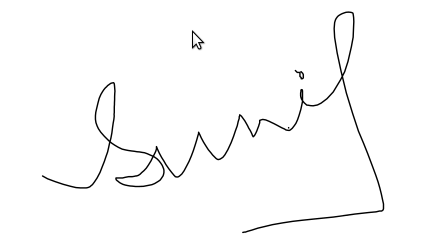
\includegraphics[width=2cm,height=1cm]{sign.png}
}
\lhead{Sunil Dhaka | Roll No.: 17817735}
\rfoot{}
\begin{document}
\section*{Report}
Code files can be viewd at https://bit.ly/3OdUirs.
\subsection*{1.}
Non linear model:
\begin{equation*}
    y(t)=\alpha_1+\alpha_2e^{\beta t} +\epsilon(t)
\end{equation*} 
Error assumption: $\epsilon(t) \sim \mathcal{N}(0,\sigma^2)$.

\begin{figure}[H]
    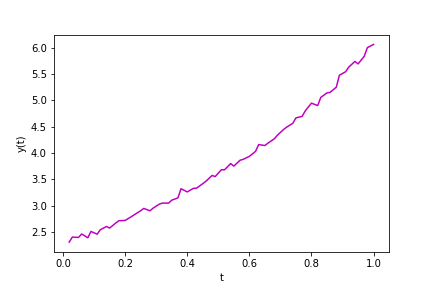
\includegraphics[]{plots/q1.png}
    \caption{plot of the data}
\end{figure}
\subsection*{2.}
The residual sum of squares is minimum for $\beta=1.307$, and value is 0.117.
\begin{figure}[H]
    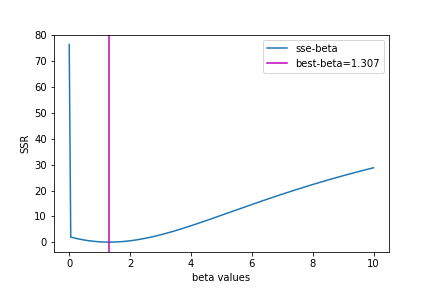
\includegraphics[]{plots/q2.png}
    \caption{the residual sum of squares as a function of $\beta$}
\end{figure}
\subsection*{3.}
Least square estimates based on Gauss-Newton methos are:
\begin{align*}
    \alpha_1&=0.848\\
    \alpha_2&=1.452\\
    \beta&=1.279
\end{align*}
\paragraph*{Initial Values:}For $\beta$, we choose the value of $\beta$ that gives minimum residual sum of squares in part-2. If we fix $\beta$ then we have a simple linear regression model. We get initial values for $\alpha_1, \alpha_2$ by OLS method. Initial values are,
\begin{align*}
    \alpha_1^{(0)}&=0.907\\
    \alpha_2^{(0)}&=1.401\\
    \beta^{(0)}&=1.306
\end{align*}
\paragraph*{Affect of starting value:}Yes, our result does get affected by initial values of parameters. But if we give Guass-Newton algorithm enough time with good enough starting values, we converge to the minima(either local or global). And if we give bad starting values, then estimates go out of bound after some time. Estimates become either really low or really high. 
\subsection*{4.}
Estimate of $\sigma^2$ can be computed using,
\begin{equation*}
    \hat{\sigma^2}=\frac{1}{n-p}(y-f(\hat{\theta}))^TV^{-1}(y-f(\hat{\theta}))
\end{equation*}
here $p=3$ and $V^{-1}=I$. After replacing, we get
\begin{equation*}
    \hat{\sigma^2}=0.00192
\end{equation*}
\subsection*{5.}
Confidence Intervals from Fisher Information matrix:
\begin{align*}
    \alpha_1&=[0.0012, 0.0025]\\
    \alpha_2&=[0.817, 0.879]\\
    \beta&=[1.364, 1.492]\\
    \sigma^2&=[1.213, 1.359]
\end{align*}

\subsection*{6.}
If the residuals are normally distributed, the data points of the normal probability plot will fall along a straight
line. Major deviations from this ideal picture reflect departures from normality. Stragglers at either end of the
normal probability plot indicate outliers, curvature at both ends of the plot indicates long or short distributional
tails, convex or concave curvature indicates a lack of symmetry, and gaps, plateaus, or segmentation in the normal
probability plot may require a closer examination of the data or model. We do not recommend that you use this
diagnostic with small sample sizes.
\begin{figure}[H]
    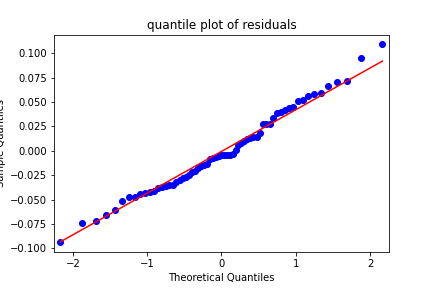
\includegraphics[]{plots/q6-1.png}
\end{figure}
\subsection*{7.}
From below residual normality tests, it is quite clear that our model residuals are approximately normal distribution.

When the row number can be equated to time period, this plot lets you see if there is a pattern across time.
\begin{figure}[H]
    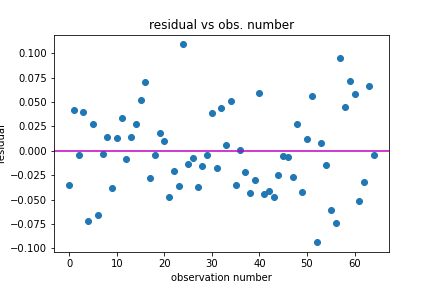
\includegraphics[]{plots/q6-2.png}
\end{figure}

This plot should always be examined. The preferred pattern to look for is a point cloud or a horizontal band. A
wedge or bowtie pattern is an indicator of nonconstant variance. A sloping or curved band signifies inadequate
specification of the model. A sloping band with increasing or decreasing variability could suggest nonconstant
variance and inadequate specification of the model.
\begin{figure}[H]
    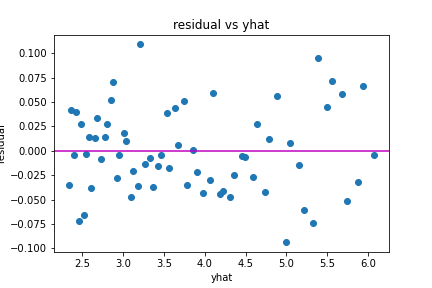
\includegraphics[]{plots/q6-3.png}
\end{figure}

This is a scatter plot of the residuals versus each independent variable. Again, the preferred pattern is a
rectangular shape or point cloud. Any nonrandom pattern may require a redefining of the model.
\begin{figure}[H]
    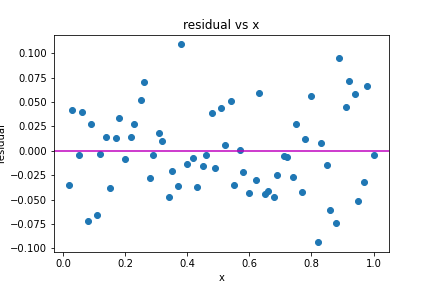
\includegraphics[]{plots/q6-4.png}
\end{figure}

Residuals histogram also seem to give approximatly normally distributed.
\begin{figure}[H]
    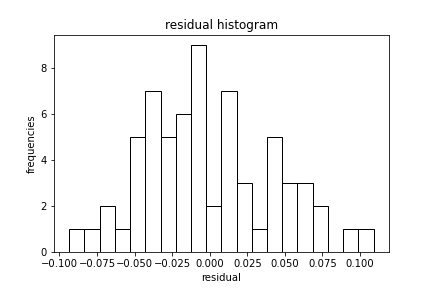
\includegraphics[]{plots/q6-5.png}
\end{figure}
\subsection*{8.}
Intial values taken from \textit{curve fit} model.

\begin{align*}
    \alpha_1^{(0)}&=0.152\\
    \alpha_2^{(0)}&=0.227\\
    \beta^{(0)}&=1.316
\end{align*}

\begin{figure}[H]
    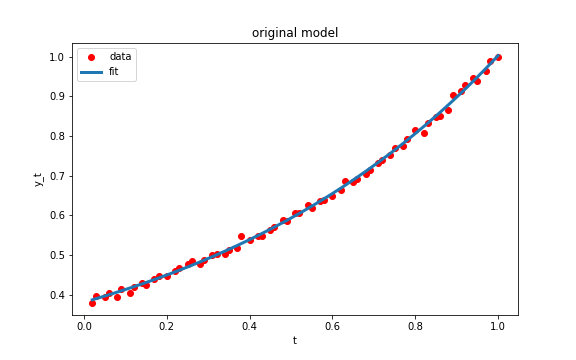
\includegraphics[]{plots/q8-1.png}
\end{figure}

\subsection*{9.}
Similar to the above model we try to solve this one also.
\begin{figure}[H]
    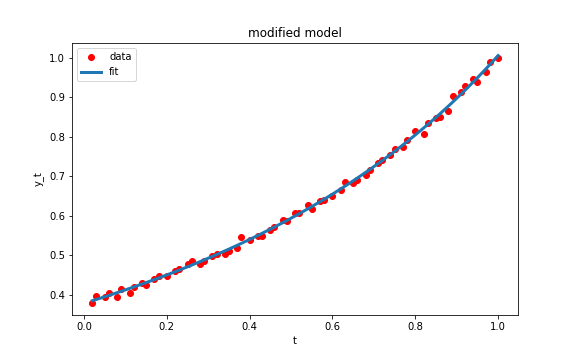
\includegraphics[]{plots/q9-1.png}
\end{figure}
\end{document}